

\section{Multi-Access Edge Computing} \label{section:MEC_evaluation}
This section will show the results of testing with the prototype for MEC and then discuss these results. Additionally, it will point out characteristics for this architecture.




\subsection{Full offloading}

\begin{table}[h!]
    \centering
    \begin{tabular}[c]{c|p{2cm}p{2cm}p{2cm}}

        Node type & Local & Near & Far \\

        Limitation          & 30 & 100 & 300  \\

        Iterations          & 0 & 900 & 9100  \\

        RTT to Local (ms)   & 0 & 30 & 170 \\

        Frequency           & 1 & 1 & 80 \\

        \hline
        \textbf{Time used (s)}       & \textbf{0} & \textbf{29.2} & \textbf{30.2} \\

    \end{tabular}
    \caption{Full offloading}
    \label{tab:MEC_full_offloading_low_frequency}
\end{table}

Table \ref{tab:MEC_full_offloading_low_frequency} shows the result of full offloading with low frequency of communication with the Far-Node.






\subsection{Partial offloading}



\begin{table}[h!]
    \centering
    \begin{tabular}[c]{c|p{2cm}p{2cm}p{2cm}}

        Node type & Local & Near & Far \\

        Limitation          & 30 & 100 & 300  \\

        Iterations          & 850 & 850 & 8300  \\

        RTT to Local (ms)   & 0 & 30 & 170 \\

        Frequency           & 1 & 1 & 80 \\

        \hline
        \textbf{Time used (s)}       & \textbf{28.0} & \textbf{29.8} & \textbf{28.0} \\

    \end{tabular}
    \caption{Partial offloading}
    \label{tab:MEC_partial_offloading_low_frequency}
\end{table}

Table \ref{tab:MEC_partial_offloading_low_frequency} shows the result of partial offloading where the Far node is doing most of the work. Frequency of communication between Local or Near node and Far node is low. 


\begin{figure}[t]
    \centering
    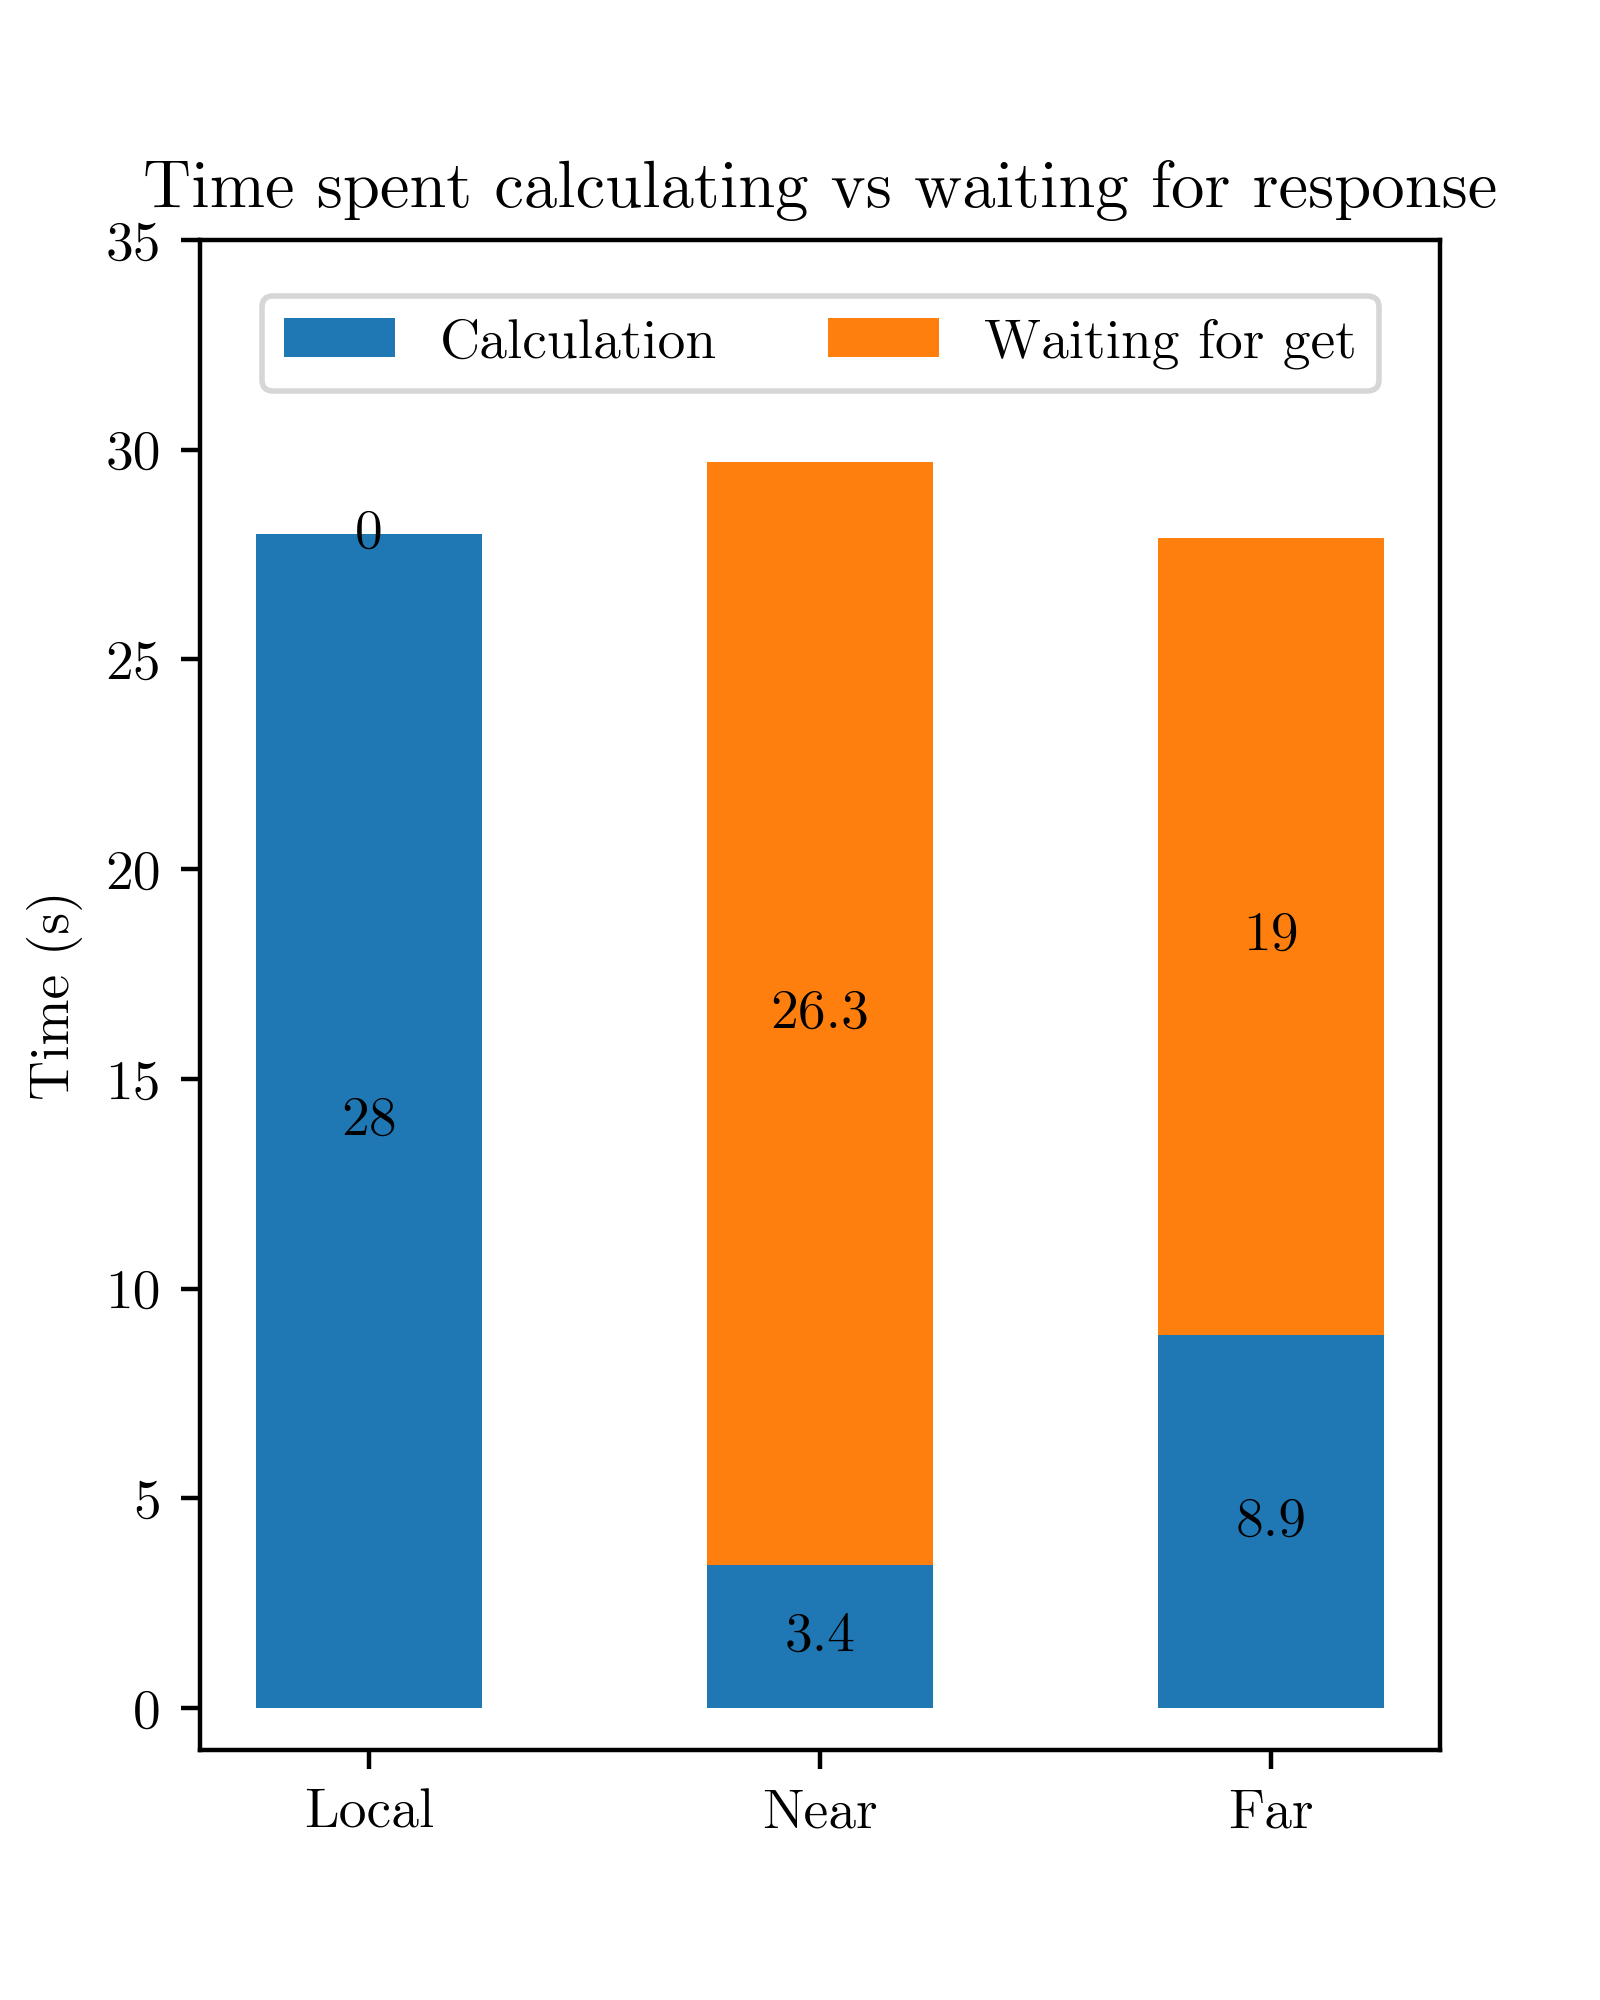
\includegraphics[scale=1]{chapters/6_evaluation/figures/MEC_Partial_bar.png}
    \caption{Illustration of how much time is spent on waiting for data due to latency when using MEC Server.}
    \label{fig:MEC_partial_bar}
\end{figure}

Figure \ref{fig:MEC_partial_bar} shows how latency affect the the total time used when we have to constantly get data from the local device. It uses the same configuration as shown in table \ref{tab:MEC_partial_offloading_low_frequency}.





\subsection{Characteristics}

\subsubsection{Control}
As discussed in section \ref{section:MEC_architecture}, the network architecture of MEC is up to the programmers. They can use NFV and SDN to control how each mobile device will use the architecture. They can, in other words, use SDN and NFV to tailor the network to the context. Since VMs can be uploaded to surrounding MEC Servers, ensuring good \textit{relocation transparency} should be trivial. Due to SDN and NFV, they could quickly redirect packets to the new MEC Server when needed. The level of \textit{migration transparency} is therefore also left to developers.

\subsubsection{Offloading}
Since MEC uses the cellular network to offload work, this architecture is well suited for IoT devices that can afford the 30ms latency. The cellular network is ubiquitous in modern society, and therefore it is optimal for IoT devices that move a lot, e.g., self-driving cars. When offloading, they have to upload something, e.g., a VM, to the MEC Server. Alternatively, they can make the MEC Server download from elsewhere. Since MEC uses VMs on the servers when offloading, the level of \textit{access transparency} is excellent. The VMs ensure that the APIs for all the nodes are the same. Since cellular networks cover such a large area, \textit{location transparency} is trivial as the device can move quite a lot of distance before any migration is needed. If a node were to fail, it is up to the developers to ensure that other resources are available to recover from the failure. In other words, the level of \textit{failure transparency} is up to the programmers.

\subsubsection{Deployment}
MEC is easily horizontally scalable, as more MEC Servers can easily be added to base stations. The only limit is how much power there is available and how much space there is available. If only a few servers are needed, then the cost is not too high either. It is also easily scalable because more VMs can be added to the MEC Server to help with offloading if needed. Another benefit of using VMs is that \textit{concurrency transparency} is easy to ensure as long as the MEC Server does not run out of resources. This is because they are in separate VMs and should not affect each other.



%offloading
%    compute 
%    storage
%distribution
%    scaling
%Control


%tabell? subsections? idk

%TODO
% Gjøre målinger med overføring av filer først. Finn data på bandwidth og pluss det på tiden.
% Gjøre målinger hvor det kreves mer samhandling mellom nodene. Vi må se latency!


%\cite{mach_mobile_2017} for hvor mye som skal offloades.!!!!
% test med 100% offload, 50% offload osv
%\begin{itemize}
 %   \item Easily scalable as we have the common interface. This makes it easy to add more vms to run more apps. So, its horizontally scalable?
%\end{itemize}